\chapter{\emph{U Network} Platform Implementation}
To achieve high concurrency in \emph{U Network} applications, we will develop a native \emph{U Network} public chain, which is highly accessible and extensible, with low latency. We expect it to be able to confirm a transactions as fast as 6 seconds and could concurrently process up to 3000 transactions per second. 
We will support high-frequency micro payments in \emph{U Network} public chain. And we will provide a easy-to-use smart contract interface. 

\section{Requirements for Blockchain Platform}
In order to achieve high adoption among users, applications require a blockchain platform that is powerful enough to meet the following requirements:
\begin{itemize}
\item {\bf high scalability}: In order to serve millions of users, a blockchain should scale up to hundreds of thousands transaction per second. As a successful tranditional centralized online shopping platform, Alibaba, on the Singles Day in 2017, the peak number of its transactions per second reached 325,000 and payment transactions reached 250,000 \cite{spencerkimball}. An application on blockchain can only be as successful if the underlying blockchain infrastructure can support an equal scale.
\item {\bf easy accessibility}: To make applications on blockchain accessible to a broader group of people, a blockchain has to offer users more friendly UI/UX which can be easily navigated. Current UI exposing information on a blockchain is intimidating for a new user, e.g. https://blockchain.info for Bitcoin and https://etherscan.io for Ethereum. Only when a blockchain is friendly for all kinds of users, can applications built on it gain more adoption.
\item {\bf low latency}: A successful blochchain infrastructure should be able to confirm a transaction within a reasonable time period. It is hard to imagine an application will be widely used if it requires 10 minutes before confirming a transaction. Either getting a coffee at Starbucks or clicking an upvote on Facebook, these all requires a respond time within seconds. In fact, the effect of latency on business success is well studied: Amazon found every 100ms of latency cost them 1\% in sales and Google found an extra 0.5 seconds in search page generation time dropped traffic by 20\% \cite{amazonlatency}. 
\item {\bf deterministic execution}: A blockchain needs to maintain a unique order of all transactions. This is particularly important for \emph{U Network}, since on \emph{U Network} the sequence of users' upvotes determine the rewards each user can get.
\end{itemize}


\section{Technical Architecture}
\begin{figure}
\centering
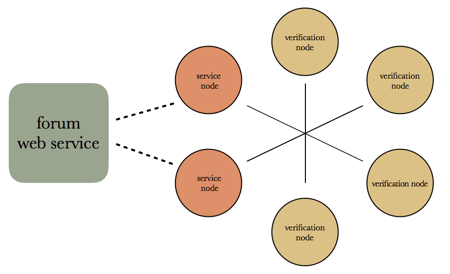
\includegraphics[width=0.8 \linewidth]{Network.png}
\caption{System Architecture}
\label{fig:system_architecture}
\end{figure}
The system architechture is shown in \ref{fig:system_architecture}. There are three major components
\begin{enumerate}
    \item ) Blockchain network verification node
    \item ) Blockchain network service node
    \item ) Web service node
\end{enumerate}
	
    Blockchain verification nodes and service nodes constitute the low level blockchain network. Verification nodes are used for verifying transactions and generating new blocks. Service nodes are designed to provide higher level service, such as block explorer, transaction search and system information search. Inside community system, service nodes are subjected to the community web service nodes, which provides necessary API for joining the community with the blockchain. Community web service nodes are user-orientated web services. It's responsible for new user registration and posting new threads. 

\section{UBFT Consensus Protocol}

\subsection{UBFT}
    UBFT stands for \emph{U network Byzantine Fault Tolerant} consensus algorithm, a novel consensus algorithm that combines the advantages of dPOS (Delegated Proof of Stake) algorithm and an improved Practical Byzantine Fault Tolerant (PBFT) algorithm\cite{pbft}. UBFT has two voting mechanisms built inside to keep the network secure from malicious attacks at all levels, while allowing all participants of the network to contribute to the security and performance of the system. 

\begin{figure}
\centering
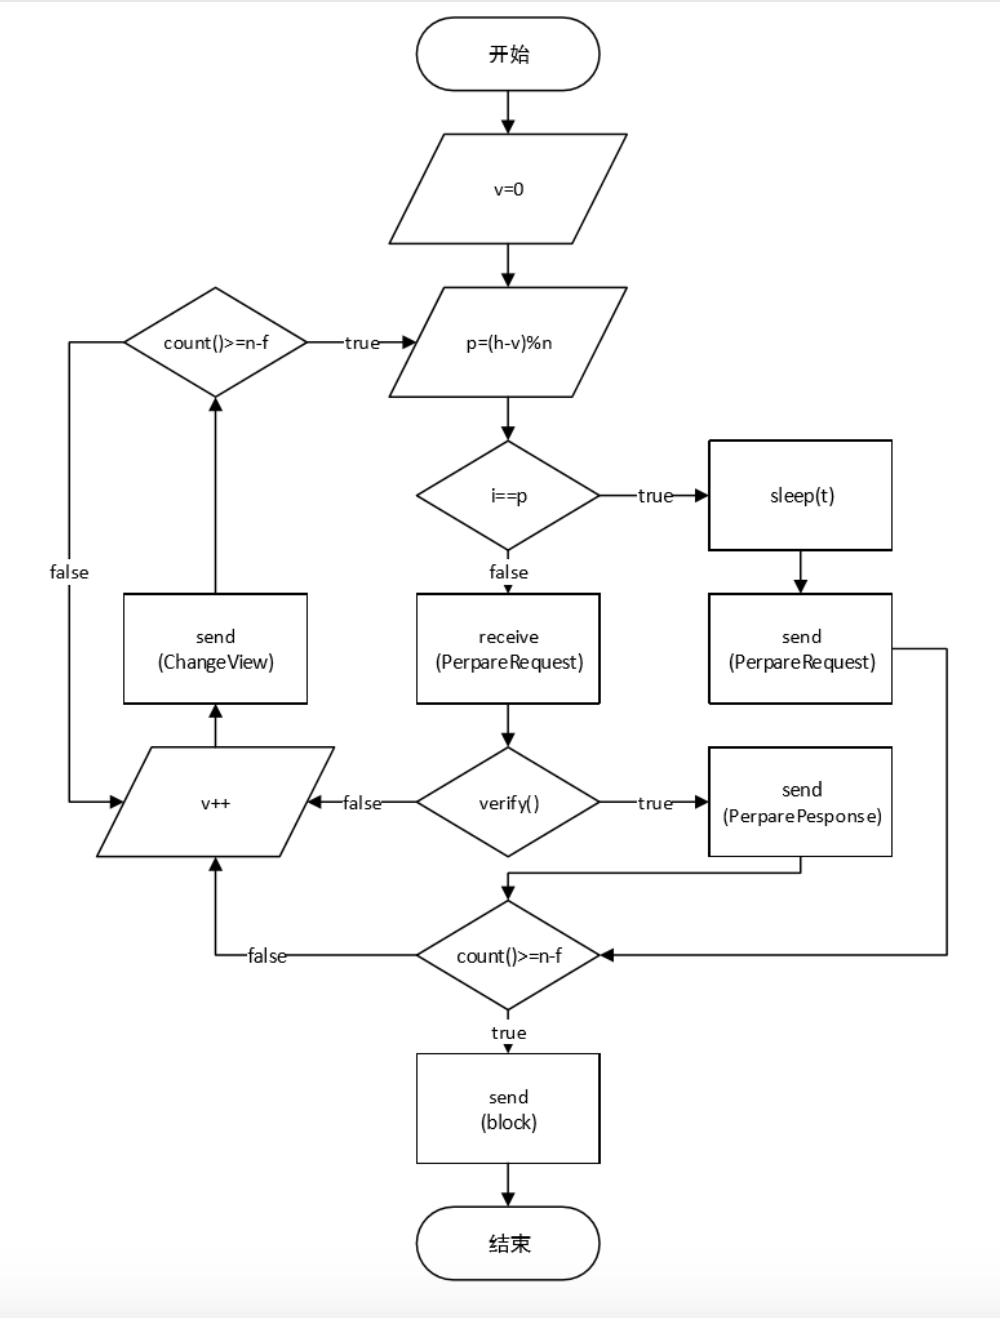
\includegraphics[width= 0.7 \linewidth]{consensus.png}
\caption{BFT Flow Chart (source: A Byzantine Fault Tolerance Algorithm\cite{neo})}
\label{fig:ubft}
\end{figure}    
    
    The overall flow is shown in Figure \ref{fig:ubft}. This algorithm have a fault tolerant rate up to 1/3. Verification node is produced by voting. Only \emph{U Network} token stakeholders have the right to vote.  UBFT has following advantages:
\begin{enumerate}
    \item ) There will be no soft-fork. One confirmation is enough for a transaction. 
    \item ) No mining is needed, energy friendly.
    \item ) Adjustable block time. We expect the block time around 6 seconds. 
    \item ) Highly concurrent in comparison to traditional blockchain. 
    \item ) No delegates needed, while improving security and performance
\end{enumerate}



\subsection{Terms Used}
    \textit{Nodes} are blockchain participants that are connected to each other by peer-to-peer network, they can be running on different hardwares and operating systems and talk to each other by \textit{gossip protocol}, which is essentially a continuous broadcast protocol with signed content. Each \textit{node} maintain a full record of the blockchain history. \textit{SPV} clients are users with public address in the network, they can be running on a web browser, mobile phones, tablets, etc. \textit{SPV} clients don't maintain full records of the whole blockchain but rather those related to themselves.

    \textit{Verifiers} are \textit{nodes} that are elected by both other \textit{nodes} and interested \textit{SPV} clients to produce new blocks each \textit{round}. There could be multiple \textit{rounds} to produce a new block if consensus is not established in the first \textit{round}.

\subsection{Assumption of Protocol}
    It is of vital importance to keep a consensus protocol safe from malicious attack in a variety of forms, and yet a quantitative analysis on this matter is hard to define. To demonstrate and measure the safety of our protocol, we'll start by making a few assumptions.
\begin{enumerate}
    \item ) The network is partially synchronous, that is, there exists an unknown upper limit to the message delay between nodes.
    \item ) There are at most 1/3 of rogue nodes in the network.
    \item ) Nodes in the network are self-interested and there's no limit as to what malicious attackers can do.
\end{enumerate}
    We make these three assumptions so that we are able to further define our protocol. Specifically, we are not, and cannot define a consensus protocol that is Byzantium Fault-Tolerant in an asynchronous setting, as indicated by the FLP Impossibility result. While we assume there exists an upper limit to the maximum delay time in the network, the protocol does not use the knowledge of its value. Compared to alternative protocols such as DPOS, which assumes a synchronous network, our protocol is more applicable in a setting where nodes are running on different hardwares and there might be huge delays in between.

    We also assume that there has to be at least 2/3 honest nodes in the system, as it's the theoretical limit of any BFT algorithm.

    The third assumption implies that to establish a safe consensus protocol, a Nash equilibrium has to be established such that any deviation from the equilibrium leads to a net loss, which could be defined economically (such as Bitcoin) or through other means.

\subsection{Security of Protocol}
    UBFT is a derived version of PBFT algorithm, therefore as long as there are more than 2/3 honest nodes in the system, it is considered secure. While the ability to tolerate at most 1/3 failed nodes seems like a degradation from POW's 1/2 allowance (such as Bitcoin), one should be aware that UBFT, like other PBFT algorithms, is able to tolerate \textbf{any failure} instead of only crash. This improvement is crucial to our overall system design since U Network is designed to be able to host a wide spectrum of applications, which may result in different failure modes.
    In simple terms, the overall structure of the protocol could be stated as following.
\begin{enumerate}
    \item  UBFT produces block at roughly 6 seconds per block.
    \item  Every time a block is to be produced, a node in the system is elected to be the producer, and only the producer will be able \& required to generate a new block.
    \item  The producer is elected in a weighted round-robin fashion, with the weight being proportional to the amount of tokens deposited by each node and the votes they received from other nodes \& SPV.
    \item  The block produced by the producer might not be recognized by 2/3 majority of the system, in which case another producer will be elected, util a new block is produced.
    \item  The liveness of the system is guaranteed by the economic incentives for the nodes to correctly generate new blocks.
    \item  The election mechanism makes it possible for end users to contribute to the security of the system and thus restricted the power of full nodes.
\end{enumerate}

\subsection{Performance}

There are some popular metrics to evaluate the performance of a certain consensus protocol, to name a few, scalability, throughput and latency, etc.

In terms of scalability, it's more like a trade-off between scalability of adding new nodes and performance of transactions processing speed, as indicated by Vukolic M in one of his recent work \cite{bft_perf}. According to Vukolic, PoW protocol has an advantage of relatively higher node scalability since PoW used entirely distributed identity management, which means each node can download the full blockchain data and start participating the protocol. This is why PoW has been adopted by many public blockchain and so-called permission-less blockchain where anybody is allowed to participate. This feature enables PoW based blockchains to involve thousands of maintaining nodes, which guaranteed its decentralization. 

BFT and its derivatives, on the other hand, could only support a limited number of full nodes, practically less than 20. This is because the more nodes involved in the BFT consensus stage, the more messages need to be transferred and slower can reach consensus. Thus BFT-based consensus can offer a good performance in a small group of replicas, which brings criticism of its centralization.

\begin{figure}
\centering
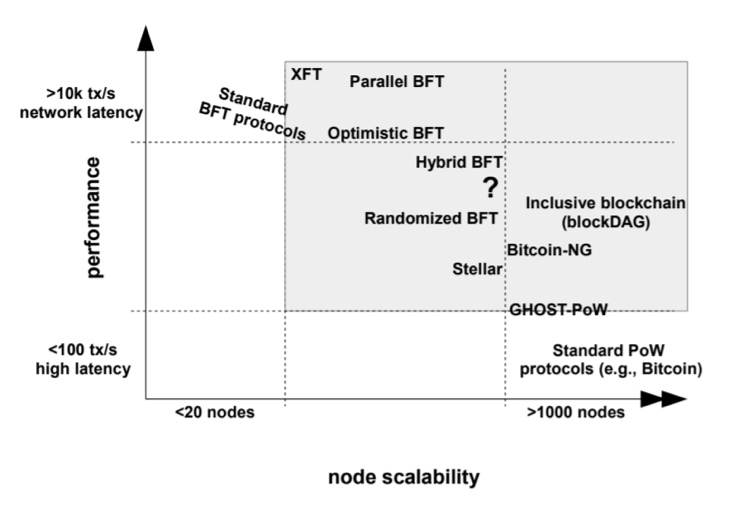
\includegraphics[width=  \linewidth]{bft_perf.png}
\caption{BFT Performance vs. Scalability}
\label{fig:bft_perf}
\end{figure}   

Based on the previous observation, UBFT tried to hit the sweet spot between the node scalability and performance. By carefully choosing the number of validation nodes, consensus can be reached in a considerable fast speed. At the same time, UBFT can also support thousands of transactions per second and matches the latency of network. In addition, the centralization could be avoided by adopting the delicate producer election process, which involve both the opinions from maintainers and platform users. By doing so, we tried to achieve an optimal balance between the scalability and the throughput performance, fit the demand of our applications and guarantee our decentralization philosophy.

%\subsection{Governance of Protocol}
%{\color{red} note: discuss how do we upgrade our consensus protocol in the future}


\section{Transaction Prococol}

%\subsection{Transaction Definition}
	In blockchain, transaction is defined as the change of ledger. It's a data structure compiled in binary that contains critical information like transaction type, transaction amount, sender address, and receiver address, time stamp, etc. All of these distinguish a transaction, and are used in both validating nodes and service nodes.  

    One major difference between \emph{U Network} blockchain and other blockchains is that we aim to make transaction types extensible, thus making it forward-compatible to applications. 
	
	Due to various types of user-generated-content products, we especially emphasize the extensibility of the system, as the growth of the decentralized \emph{U Network} could be booming one day. Therefore, by making transaction types extensible, we guaranteed the whole network is extensible without the need to change core internet protocol and consensus algorithm or storage structures.
	
	The system will support following major transaction types based on different scenario: 
	
	\begin{enumerate}
	\item )Asset register: used for coin mint
	\item )Asset publish: allocate users digital assets
    \item )Asset transfer: traditional UTXO transfer
    \item )Smart contract deploy: deploy compiled smart contract byte code to block chain
    \item )Smart contract message call: call deployed smart contract
    \item )Asset lock down: asset owner can lock the blockchain height
	\end{enumerate}
	
In order to defend against double-spent attack, all the pending transactions need to be confirmed sequentially in a deterministic way. Each validating node will have a pool of unconfirmed transactions. Given the efficiency of UBFT consensus algorithm, each verification node can verify up to 3000 transactions within 6 seconds of block time. To put it in another word, the blockchain can concurrently process 3000 transactions while keeping the transaction flow sequential. 



\section{Content Storage and Search}
\emph{U Network} internally leverages the IPFS (Inter Planetary File System \cite{ipfs}) for storing the content. IPFS is a distributed file system that seeks to connect all computing devices with the same system of files. In some ways, this is similar to the original aims of the Web, but IPFS is actually more similar to a single bittorrent swarm exchanging git objects. With IPFS, any content published in the IPFS network will be persistented forever, and accessed freely, easily and efficiently without being worried about the link expiration like HTTP. 

Meanwhile, on top of the IPFS storage, an abstract layer will be implemented in \emph{U Network} platform, to provide stable APIs to APP layers in service node, so it will easily plugin any other decentralized content storages, like Genero, into \emph{U Network} platform.

\subsection{Content Creation and Storage}
Once a piece of content is created in the \emph{U Network}, the content will be stored in IPFS and the hash to the content is returned, which will be used later for addressing. 

In the \emph{U Network}, the content address (the IPFS hash of the content) will be indexed in a smart contract. Every creation of a content will also result into a smart contract creation on the blockchain. The smart contract will have below states in the contract storage:
\begin{itemize}
\item The IPFS hash of the content.
\item The content creator's address. 
\item A list of upvoters' addresses, in sequential order.
\item A list of downvoters' addresses, in sequential order.
\item \emph{U Network} token balance. Voters' token balance used for voting will be transferred in and locked for delayed settlement. The settlement will be on demand performed per the settlement business rule, which is built-in in the smart contract.
\end{itemize}

\subsection{Content Search}

All the content created by \emph{U Network} will be grouped in an IPFS directory. There will also be an indexing file, mapping any content hash to the corresponding smart contract address. With this design, the browser will easily load the contents and their associated voters info. 

\subsection{Improvements}

A smart contract storing the content related info will be on the main blockchain initially. However, to achieve better scalability, \emph{U Foundation} plans to incorporate the state channel mechanism into \emph{U Network} platform at the next stage, like Aeternity. The content smart contract will then be created in the state channels. It will gain the below benefits using state channel:
\begin{itemize}
\item Activities on different content will be processed in parallel, and confirmed immediately.
\item It will keep the main blockchain efficient and clean.
\end{itemize}


\section{Token Incentive for Resources}

%Applications on blockchains consume three major types of resources:
%\begin{itemize}
%\item storage
%\item computation
%\item bandwidth
%\end{itemize}

\subsection{Storage Costs}
%{\color{red} note: Are we going to use IPFS for storage? If so, we need to discuss how.}
As a content blockchain platform, we need a significant amount of storage to store user-generated contents. These contents can take a large amount of space, especially for multi-media contents like vedios or pictures. These contents need to be stored in distributed network on participant nodes. Nodes who contribute storage spaces will be rewarded based on how much space they are providing.

\subsection{Bandwidth Costs}
The contents in \emph{U Network} will finally consumed by readers. To distribute contents to readers, network bandwidth will be consumed. To motivate paticipant nodes to relay contents to readers, we will account the bandwidth each relay nodes contribute and reward them with U Network tokens.

\subsection{Computation Costs}
All blockchain systems need nodes to verify transactions on top of it. \emph{U Network} will reward all nodes participating verification of a transaction when a transaction is successfully added to the public ledger, thus all nodes have the incentive to become a legit verification node. 
